%%%%%%%%%%%%%%%%%%%%%%%%%%%%%%%%%%%%%%%%%
% Beamer Presentation
% LaTeX Template
% Version 1.0 (10/11/12)
%
% This template has been downloaded from:
% http://www.LaTeXTemplates.com
%
% License:
% CC BY-NC-SA 3.0 (http://creativecommons.org/licenses/by-nc-sa/3.0/)
%
%%%%%%%%%%%%%%%%%%%%%%%%%%%%%%%%%%%%%%%%%

%----------------------------------------------------------------------------------------
%	PACKAGES AND THEMES
%----------------------------------------------------------------------------------------

\documentclass[14pt,handout]{beamer}
%%\documentclass[14pt]{beamer}

\mode<presentation> {

% The Beamer class slide themes
\usetheme{Madrid} %i was using this one

% Beamer class color themes

%\usecolortheme{albatross}

%\setbeamertemplate{footline} % To remove the footer line in all slides uncomment this line
%\setbeamertemplate{footline}[page number] % To replace the footer line in all slides with a simple slide count uncomment this line

%\setbeamertemplate{navigation symbols}{} % To remove the navigation symbols from the bottom of all slides uncomment this line
}

\usepackage{graphicx} % Allows including images
\usepackage{booktabs} % Allows the use of \toprule, \midrule and \bottomrule in tables
\usepackage{hyperref}
\usepackage{helvet}
\usepackage[T1]{fontenc}
\usepackage{textcomp}

%----------------------------------------------------------------------------------------
%	TITLE PAGE
%----------------------------------------------------------------------------------------

\title[Probability and Models]{Statistical Probability and Models} % The short title appears at the bottom of every slide, the full title is only on the title page

\author{C. Ryan Campbell} % Your name
\institute[Duke] % Your institution as it will appear on the bottom of every slide, may be shorthand to save space
{
Duke University \\ % Your institution for the title page
\medskip
\textit{c.ryan.campbell@duke.edu} % Your email address
}
\date{28 Nov 2017} % Date, can be changed to a custom date

\begin{document}

\begin{frame}
\titlepage % Print the title page as the first slide
\end{frame}

%------------------------------------------------
\begin{frame}
\frametitle{Project Updated}
\begin{itemize}
	\item<+-> Still Grading Rough Drafts - Done by Thursday
	\item<+-> Presentations are \underline{next week}
	\item<+-> Present what you have, should be more polished than the rough draft
	\item<+-> 20 minutes per group presentation
	\item<+-> 5min intro, 5min per member
	\item<+-> Order?
\end{itemize}
\end{frame}


\begin{frame}
\frametitle{Overview} % Table of contents slide, comment this block out to remove it
\tableofcontents % Throughout your presentation, if you choose to use \section{} and \subsection{} commands, these will automatically be printed on this slide as an overview of your presentation
\end{frame}

%----------------------------------------------------------------------------------------
%	PRESENTATION SLIDES
%----------------------------------------------------------------------------------------

%------------------------------------------------
\begin{frame}
\frametitle{This Week's Goals}
\begin{itemize}
	\item<+-> Understand p-values \& adjustments
	\item<+-> Learn about Maximum Likelihood
	\item<+-> Learn about Bayes Theorem \& Bayesian Probability
\end{itemize}
\end{frame}

%------------------------------------------------
\section{Probability}
%------------------------------------------------

%------------------------------------------------
\begin{frame}
\frametitle{Probability}
\begin{itemize}
	\item<+-> ``Odds'' that some event occurs
	\item<+-> Bounded from 0 to 1
	\item<+-> Usually expressed as a fraction or percent
	\item<+-> Often using the notation: Pr(event) or P(event)
\end{itemize}
\end{frame}

%------------------------------------------------
\subsection{And versus Or}
%------------------------------------------------

%------------------------------------------------
\begin{frame}
\frametitle{Or}
\begin{itemize}
	\item<+-> Probabilities of multiple events can be combined
	\item<+-> ``Or'' condition
	\item<+-> Probability either thing happens: A or B
	\item<+-> when A and B are independent and mutually exclusive:
	\item<+-> Pr(A or B) = Pr(A) + Pr(B)
\end{itemize}
\end{frame}

%------------------------------------------------
\begin{frame}
\frametitle{Or}
\begin{itemize}
	\item<+-> Probabilities of multiple events can be combined
	\item<+-> ``Or'' condition
	\item<+-> when A and B are independent and \underline{not exclusive}:
	\item<+-> Pr(A or B) = Pr(A) + Pr(B) - Pr(A \& B)
\end{itemize}
\end{frame}

%------------------------------------------------
\begin{frame}
\frametitle{And}
\begin{itemize}
	\item<+-> Probabilities of multiple events both occuring can be combined
	\item<+-> ``And'' condition
	\item<+-> Probability both things happen, A \& B
	\item<+-> When A \& B are independent:
	\item<+-> Pr(A \& B) = Pr(A) * Pr(B)
	\item<+-> ``And'' is commutative:
	\item<+-> Pr(B \& A) = Pr(A \& B)
\end{itemize}
\end{frame}

%------------------------------------------------
\begin{frame}
\frametitle{Conditional Probabilities}
\begin{itemize}
	\item<+-> Probabilities of event A \underline{given} event B
	\item<+-> Probability of A if we know B has occured
	\item<+-> When B happens, how likely is it that A happens
	\item<+-> Numerator = Pr(A \& B)
	\item<+-> Denominator = Pr(B)
	\item[] \underline{Pr(A \& B)}
	\item[] Pr(B)
\end{itemize}
\end{frame}

%------------------------------------------------
\begin{frame}
\frametitle{Some Quick Math}
\begin{itemize}
	\item[] Pr(B\textsubscript{1} given A) = ?
	\item[] Pr(B\textsubscript{2} given A) = ?
	\item[] Pr(A given B\textsubscript{2}) = ?
	\begin{center}
	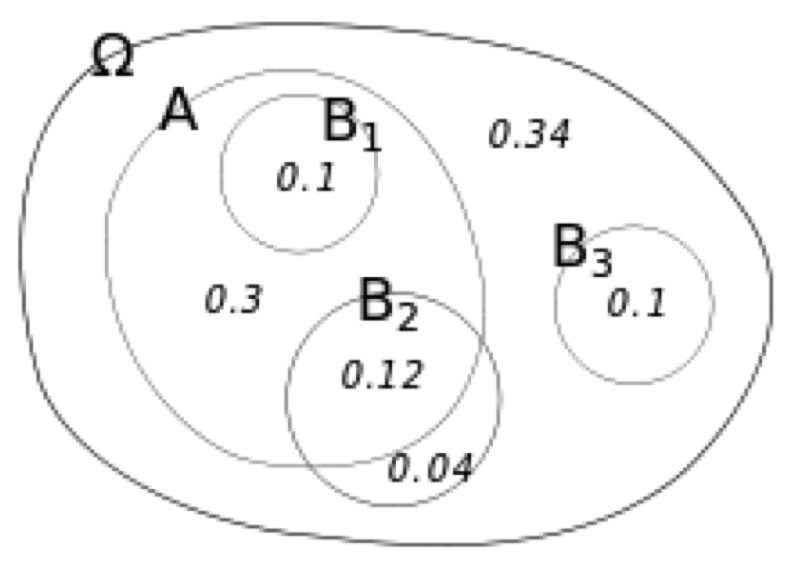
\includegraphics[width=.7\textwidth]{images_20171128_condtionalprobs.png}
	\end{center}
\end{itemize}
\end{frame}

%------------------------------------------------
\begin{frame}
\frametitle{Some Quick Math}
\begin{itemize}
	\item[] Pr(B\textsubscript{1} given A) = .1/.3 = .333
	\item[] Pr(B\textsubscript{2} given A) = .12/.3 = .4
	\item[] Pr(A given B\textsubscript{2}) = .12/(.12 + .04) = .75
	\begin{center}
	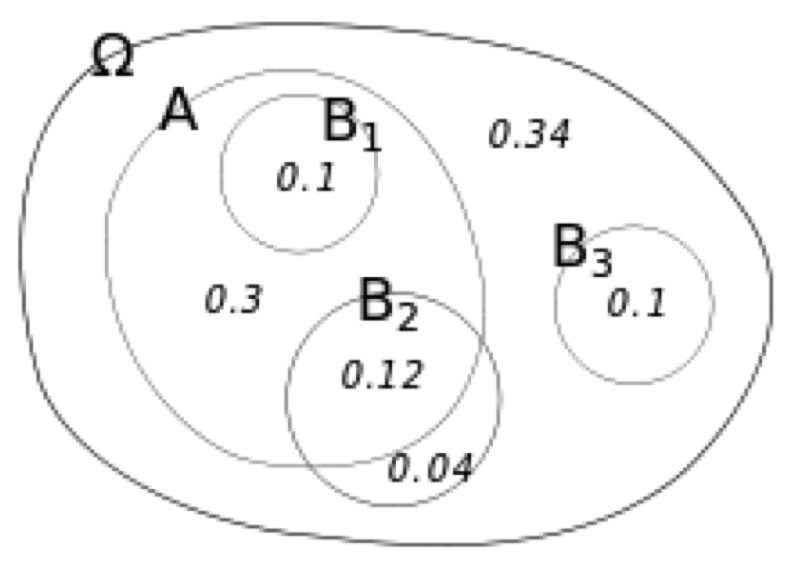
\includegraphics[width=.7\textwidth]{images_20171128_condtionalprobs.png}
	\end{center}
\end{itemize}
\end{frame}


%------------------------------------------------
\section{P-Values}
%------------------------------------------------

%------------------------------------------------
\begin{frame}
\frametitle{P-Value}
\begin{itemize}
	\item<+-> What is a P-Value?
\end{itemize}
\end{frame}

%------------------------------------------------
\begin{frame}
\frametitle{P-Value}
In statistical hypothesis testing, the p-value or probability value is the probability for a given statistical model that, when the null hypothesis is true, the statistical summary (such as the sample mean difference between two compared groups) would be the same as or of greater magnitude than the actual observed results.
\end{frame}

%------------------------------------------------
\begin{frame}
\frametitle{P-Value}
\begin{itemize}
	\item<+-> Probability of the data (or greater ``magnitude'' data)
	\item<+-> Given that the Null Hypothesis is true
	\item<+-> Only \textit{pvalue}\% of the time, if treatment and control are equal, would you expect data this different
\end{itemize}
\end{frame}

%------------------------------------------------
\section{Hypothesis Testing}
%------------------------------------------------

%------------------------------------------------
\begin{frame}
\frametitle{Hypothesis Testing}
\begin{itemize}
	\item<+-> Need the context of Hypothesis testing for p-values to have meaning
	\item<+-> H0: Group A = Group B
	\item<+-> H1: Group A \textit{does not equal} Group B
\end{itemize}
\end{frame}

%------------------------------------------------
\begin{frame}
\frametitle{Hypothesis Testing}
\begin{itemize}
	\item<+-> We assume H0 is true
	\item<+-> Compare Group A and Group B
	\item<+-> The p-value measures how likely it is the differences between A and B are due to chance
	\item<+-> A lower p-value gives more power to \underline{reject H0}
\end{itemize}
\end{frame}

%------------------------------------------------
\begin{frame}
\frametitle{Let's Try an Example}
\begin{itemize}
	\item Run a comparison of means in R
	\item Compare two random sets of data with a t-test, using
	\ttfamily
	\footnotesize
	\begin{block}{}
	\item[] > rnorm()
	\item[] > t.test() 
	\end{block}
	\normalsize
	\sffamily
	\item mean 0, stdev 1, n 10
	\item What is your p-value?
\end{itemize}
\end{frame}

%------------------------------------------------
\begin{frame}
\frametitle{Let's Try an Example}
\begin{itemize}
	\item Run a comparison of means in R
	\item Compare two random sets of data with a t-test, using
	\ttfamily
	\footnotesize
	\begin{block}{}
	\item[] > rnorm()
	\item[] > t.test() 
	\end{block}
	\sffamily
	\item[] mean of 0
	\item[] stdev of 1
	\item[] n of 10
	\item What is your p-value?
\end{itemize}
\end{frame}

%------------------------------------------------
\begin{frame}
\frametitle{Let's Try an Example}
\begin{itemize}
	\item<+-> Is H0 true or false?
	\item<+-> Did anyone get a p-value suggesting otherwise?
	\item<+-> Why?
\end{itemize}
\end{frame}

%------------------------------------------------
\begin{frame}
\frametitle{Let's Try an Example}
\begin{itemize}
	\item<+-> What is the distribution of p-values over many tests?
	\item<+-> How many tests is a single DESeq analysis?
	\item<+-> Use a for loop and R to replicate the example, but on a DESeq scale
\end{itemize}
\end{frame}

%------------------------------------------------
\begin{frame}
\frametitle{Let's Try an Example}
\begin{itemize}
	\item[] Use a for loop and R to replicate the example, but on a DESeq scale
	\ttfamily
	\footnotesize
\begin{block}{}
	\item[] for (n in 1:high number) \{
	\item[] generate p-values
	\item[] \}
\end{block} 
	\normalsize
	\sffamily
	\item[] How do you save all your p-values?
\end{itemize}
\end{frame}

%------------------------------------------------
\begin{frame}
\frametitle{Let's Try an Example}
\begin{itemize}
	\item<+-> Visualize the distribution of p-values
	\item<+-> What do you see?
\end{itemize}
\end{frame}

%------------------------------------------------
\begin{frame}
\frametitle{Let's Try an Example}
\begin{itemize}
	\item[] My code:
	\ttfamily
	\footnotesize
\begin{block}{}
	\item[]  pvals <- 1:10000
	\item[]
	\item[]  for (n in 1:10000) \{
	\item[]  pvals[n] <- t.test(rnorm(10,0,1),rnorm(10,0,1),var.equal = T)\$p.value
	\item[]  \}
	\item[]
	\item[]  hist(pvals)
\end{block}
\begin{center}
	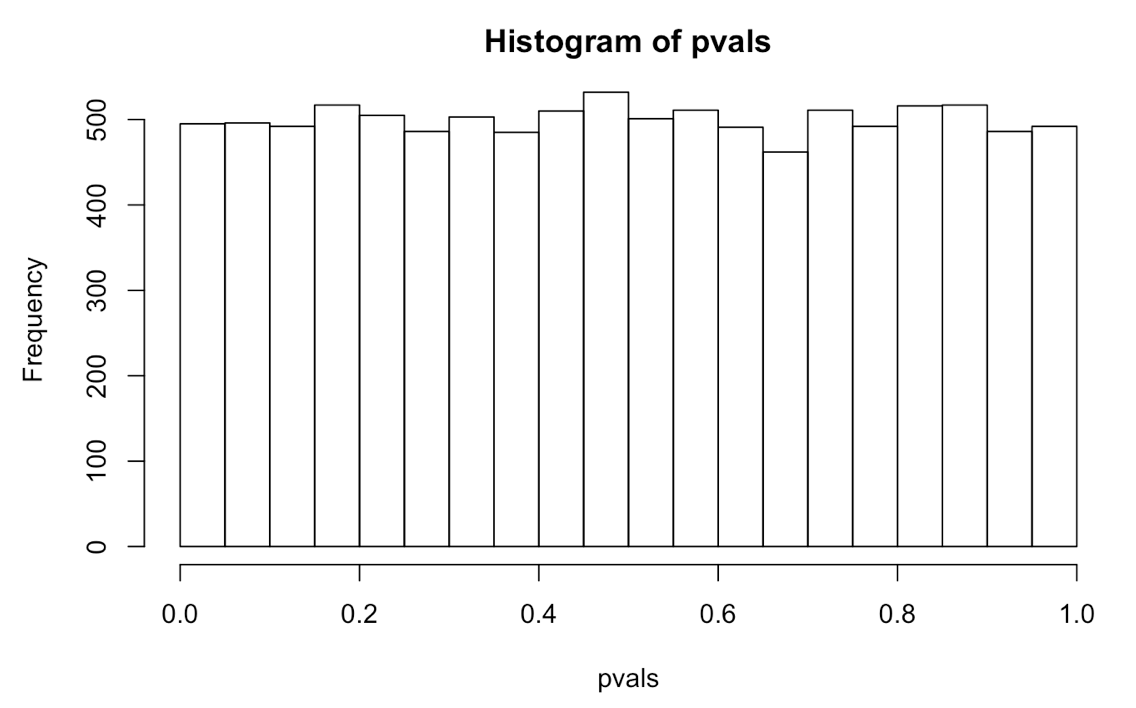
\includegraphics[width=0.3\textwidth]{images_20171128_R_pvals.png}
\end{center}
\end{itemize}
\end{frame}

%------------------------------------------------
\subsection{Multiple Tests}
%------------------------------------------------

%------------------------------------------------
\begin{frame}
\frametitle{Multiple Tests: xkcd}
	\begin{center}
	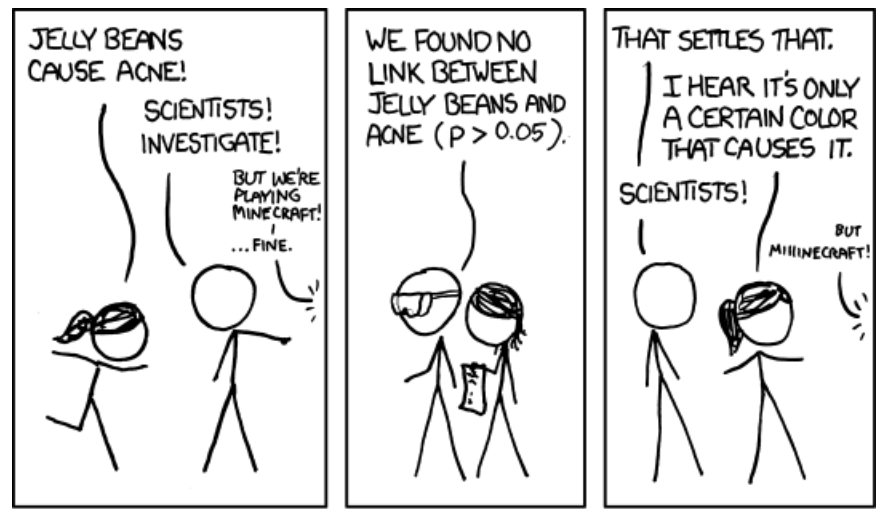
\includegraphics[width=1.0\textwidth]{images_20171128_xkcd_pval1.png}
	\end{center}
\end{frame}

%------------------------------------------------
\begin{frame}
\frametitle{Multiple Tests: xkcd}
	\begin{center}
	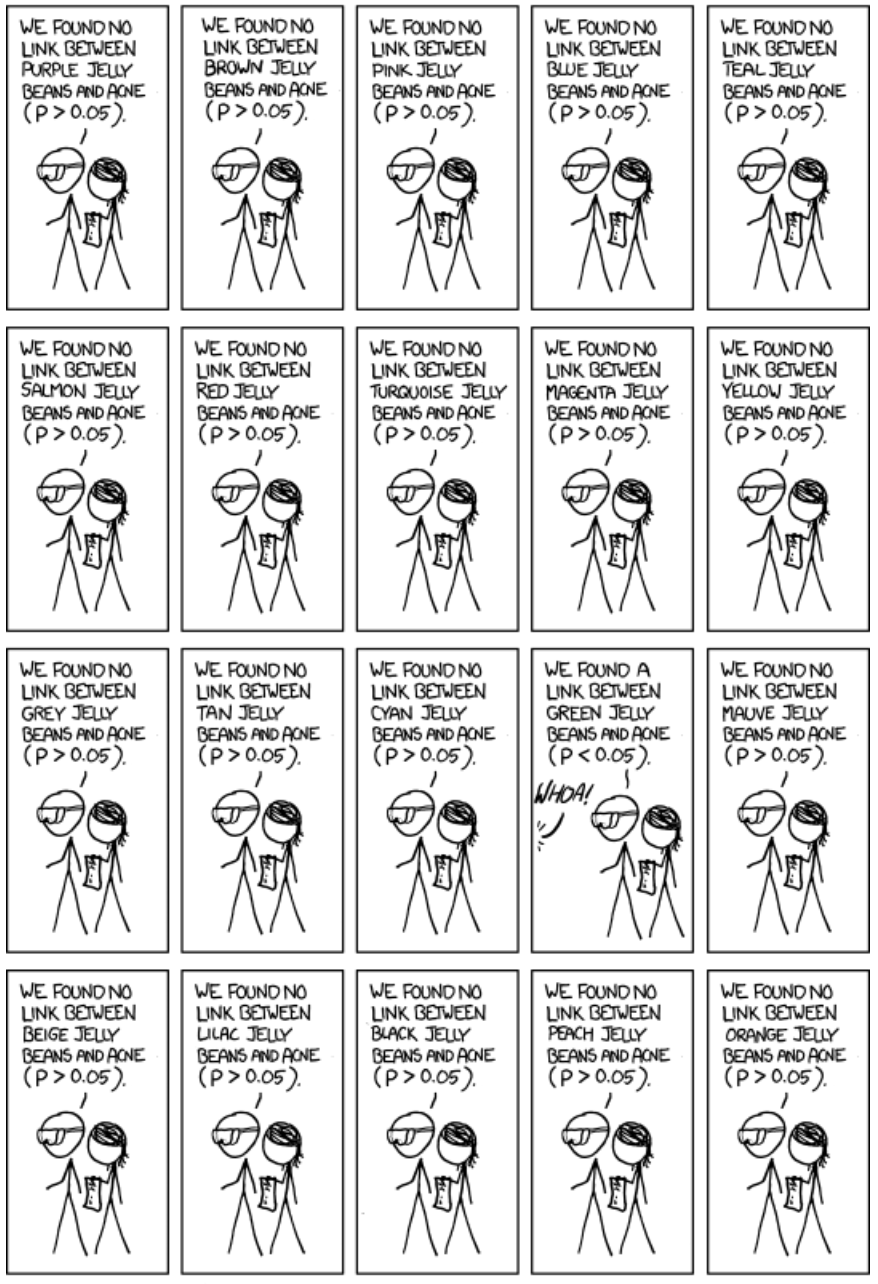
\includegraphics[width=.45\textwidth]{images_20171128_xkcd_pval2.png}
	\end{center}
\end{frame}

%------------------------------------------------
\begin{frame}
\frametitle{Multiple Tests: xkcd}
	\begin{center}
	
\includegraphics[width=.6\textwidth]{images_20171128_xkcd_pval3.png}
	\end{center}
\end{frame}

%------------------------------------------------
\begin{frame}
\frametitle{Multiple Tests}
\begin{itemize}
	\item<+-> If you conduct 10,000 t-tests
	\item<+-> AND the null hypothesis is true
	\item<+-> How many will yield a p-value capable of rejecting the null
	\item<+-> at alpha = 0.05?
	\item<+-> at alpha = 0.01?  
\end{itemize}
\end{frame}

%------------------------------------------------
\begin{frame}
\frametitle{Multiple Tests: Solutions}
\begin{itemize}
	\item<+-> What do we do?
	\item<+-> How do you take this into account?
	\item<+-> Bonferroni corrections
	\item<+-> Adjusted P-Values
	\item<+-> Permutation tests
\end{itemize}
\end{frame}


%------------------------------------------------
\subsection{Bonferroni Correction}
%------------------------------------------------

%------------------------------------------------
\begin{frame}
\frametitle{Bonferroni Correction}
\begin{itemize}
	\item<+-> Very simple approach
	\item<+-> Combine your alpha level (0.05)
	\item<+-> With the number of tests (10,000)
	\item<+-> 0.05/10,000 is the altered p-value level
	\item<+-> per-test alpha = 5x10\textsuperscript{-6}
\end{itemize}
\end{frame}

%------------------------------------------------
\begin{frame}
\frametitle{Bonferroni Correction}
\begin{itemize}
	\item<+-> Pros and Cons:
	\item<+-> + Easy to apply
	\item<+-> + Flexible for number of tests
	\item<+-> - Overly Conservative (will accept false nulls)
	\item<+-> - Assumes independence
\end{itemize}
\end{frame}

%------------------------------------------------
\subsection{Adjusted P-Value}
%------------------------------------------------

%------------------------------------------------
\begin{frame}
\frametitle{Adjusted P-Value}
\begin{itemize}
	\item<+-> More statistically complex
	\item<+-> Aims to reduce FDR - False Discovery Rate
	\item<+-> False Discovery - all of the random samples we drew earlier with T-tests that fell below 0.05
	\item<+-> This is why you'll want to rely on padj from DESeq
\end{itemize}
\end{frame}

%------------------------------------------------
\begin{frame}
\frametitle{Adjusted P-Value: Example}
\begin{itemize}
	\item<+-> Benjamini-Hochberg procedure
	\item<+-> Sort results by p-value
	\item<+-> Assign each test a BH score of:
	\item<+-> (rank/N of tests) * acceptable FDR
\end{itemize}
\end{frame}

%------------------------------------------------
\begin{frame}
\frametitle{Adjusted P-Value: Example}
\begin{itemize}
	\item<+-> For the ``best'' results (lowest P-Values) you should see:
	\item<+-> p-value less than BHscore
	\item<+-> Find the worst p-value that is still less than its BHscore
	\item<+-> All tests below that are significant
\end{itemize}
\end{frame}

%------------------------------------------------
\begin{frame}
\frametitle{Adjusted P-Value: Example}
\begin{itemize}
	\item Find the worst p-value that is still less than its BHscore
	\item That test and all tests below that are significant:
	\begin{center}
	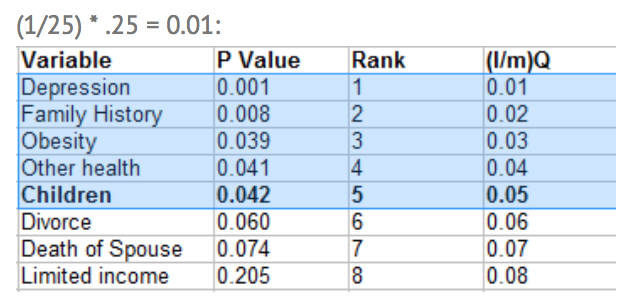
\includegraphics[width=.7\textwidth]{images_20171128_BHscore.png}
	\end{center}
\end{itemize}
\end{frame}

%------------------------------------------------
\subsection{Permutation Tests}
%------------------------------------------------

%------------------------------------------------
\begin{frame}
\frametitle{Permutation Test}
\begin{itemize}
	\item<+-> A form of resampling your data
	\item<+-> (other forms are Jackknifing or Bootstrapping)
	\item<+-> You re-label your samples (control v. experimental)
	\item<+-> Rerun the analysis
	\item<+-> See where the actual test's p-value falls on the range of p-values this produces
\end{itemize}
\end{frame}

%------------------------------------------------
\begin{frame}
\frametitle{Permutation Test}
\begin{itemize}
	\item<+-> Two possible outcomes:
	\item<+-> 1) The instance with the correct labels falls in the middle of the distribution
	\item<+-> 2) The instance with the correct labels is a significant outlier
	\item<+-> What do each of these mean?
\end{itemize}
\end{frame}

%------------------------------------------------
\begin{frame}
\frametitle{Multiple Tests: xkcd}
How would each correctional method have dealt with our jelly bean problem?
\begin{center}
	
\includegraphics[width=.6\textwidth]{images_20171128_xkcd_pval3.png}
\end{center}
\end{frame}

%------------------------------------------------
\section{Models}
%------------------------------------------------

%------------------------------------------------
\subsection{Maximum Likelihood}
%------------------------------------------------

%------------------------------------------------
\subsection{Bayes Rule}
%------------------------------------------------

%------------------------------------------------
\section{ML versus Bayes Rule: An Example}
%------------------------------------------------


%------------------------------------------------
\begin{frame}
\Huge{\centerline{The End}}
\end{frame}

%----------------------------------------------------------------------------------------

\end{document} 